
No practical amount of data can distinguish between two distributions, thus instances of GBS can not be proven to come from GESIS. However, machine learning allows to infer the conditional probability of \textit{'GBS participant is representative'} given the survey data within a probabilistic framework. A well-defined learning problem involves a number of design choices, including selecting the target function to be learned, a representation for this target function, and an algorithm to learn from the source of training experience [2]. This chapter covers the theoretical aspects of the MRS procedure introducing positive-unlabeled learning in addition to traditional machine learning.

\section{Terminology and Definitions}

Key terminology and destinctions made in the field of survey analytics are defined in this section. When learning from biased data, basic design issues and approaches to discriminative learning must be adjusted. The role of noise in the bias-variance decomposition will be analyzed and further broken down. Discriminative learning then uses techniques to address high variance.

\subsection{Sampling Bias}

Sampling bias is often referred to as selection bias or sample selection bias. I will stick to the more descriptive term sampling bias. It underlines the fact that the bias arises in how the data was sampled. Also, the use of the term becomes less ambiguous, because there exists another notion of selection bias in the context of model selection. This type of bias is usually referred to as bad generalization, where the performance of the selected hypothesis is overly optimistic. [input: convenience sampling]

Although one could employ a census to measure the entire population, it is more common to take a sample of the population. A properly designed probability sample (see probability sampling) can be used to make estimates for not only the sample itself, but also for the underlying population from which it was selected. A probability sample is one in which each element of the (underlying) population has a known and non-zero chance of being selected. That is, every person has a chance to be included in the study and have his or her characteristics, opinions, etc., become part of the data. It should be noted that everyone does not have to have an equal chance of being selected – just a known non-zero chance of being selected. 
Probability samples have several desirable characteristics. They enable us to put a margin of error or confidence interval on our estimates – essentially a measure of how accurate the estimate is compared to the same estimate calculated on the full population. Probability samples make it possible to not only compare the sample to the population, but also to compare a sample from one population to a sample from another population,

\subsection{Representative Sample}

Variables considered in the study must accurately reflect the populations characteristics. Some examples include sex, age, education level, socioeconomic status or marital status. Consider a randomly chosen survey participant, i.e. an instance of GBS or GESIS. It is usually difficult to draw a simple random sample from the population, due to cost and practical considerations such as no comprehensive sampling frame available.

\begin{figure}[ht]
	\begin{center}
		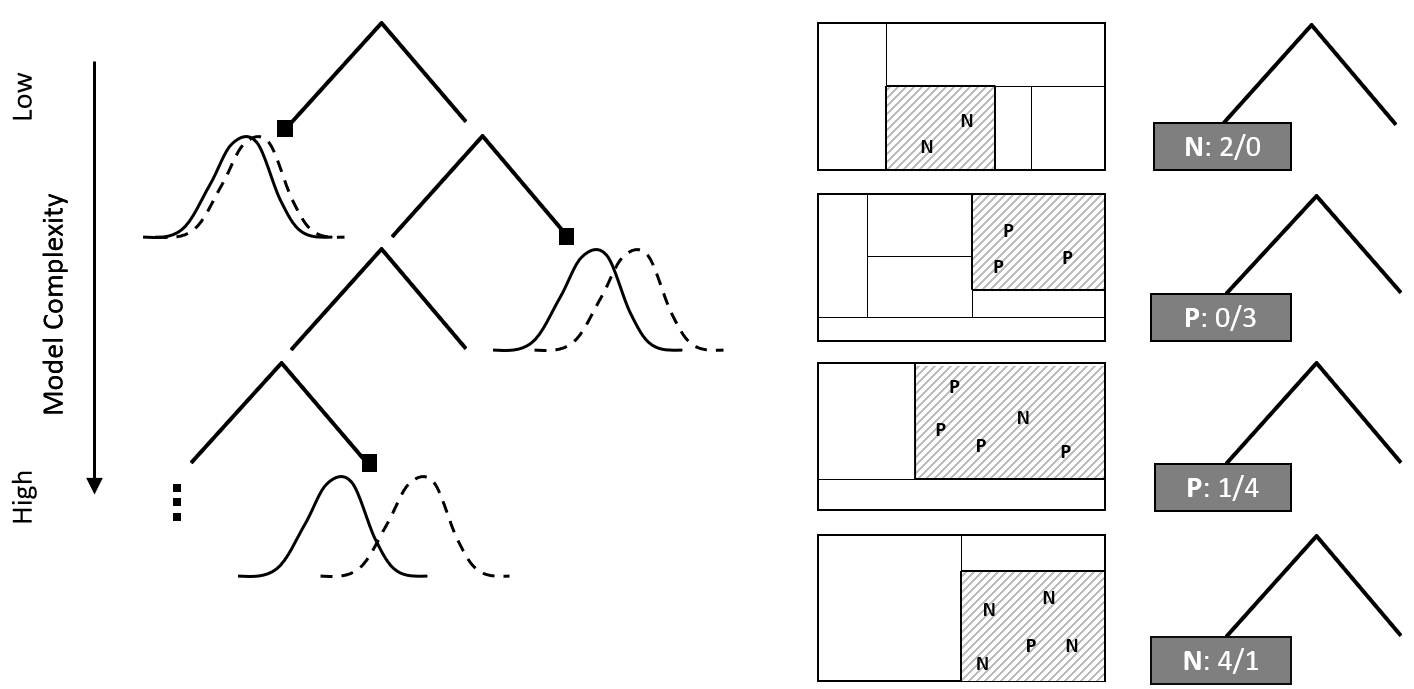
\includegraphics[scale=0.40,angle=0]{fig/tree3}
		\label{project}
		\caption{.}
	\end{center}
\end{figure}

\subsection{The Problem of Overfitting}

Overfitting stands out as one of the biggest challenges for machine learning. It is not exclusive to machine learning but rather a fundamental problem across science and is at the very heart of the dangers of statistical inference. Hypothesis \(h\) in \(H\) overfits training data if there exists an alternative hypothesis \(\bar{h}\) in \(H\) such that \(errorTrain(h) < errorTrain(\bar{h})\) and \(errorD(h) > errorD(\bar{h})\), where \(errorTrain(h):=\) error of hypothesis \(h\) over training data and \(errorD(h):=\) error over entire distribution \(D\) of data. A hypothesis overfits the training examples if some other hypothesis that fits the training examples less well actually performs better over the entire distribution of instances [1].

When overfitting occurs, the learned hypothesis is very good at calculating the answers for the given data, but much less so for new instances it encounters. In a sense, the machine learning algorithm has become fixated on unimportant features of the training data overlooking the big picture. It often occurs when the algorithm has too many options to play with in designing its mappings, an approximation of the target function. The freedom to tune parameters and add complexity until it exactly matches the training data, rather than looking for large, systematic patterns leads to high variance [6].

The expected prediction error at any given data point \(x_0\), the generalization error, can be decomposed as follows [5]: 
\begin{align*}
Err(x_o) &= \EX[(Y - \bar{f}(x_0))^2 \mid X = x_0] \\
& =  \sigma^2_\epsilon + [\EX\bar{f}(x_0) - f(x_0)]^2 + \EX[\bar{f}(x_0) - \EX\bar{f}(x_0)]^2\\
& =  \sigma^2_\epsilon + Bias^2(\bar{f}(x_0)) + Var(\bar{f}(x_0)) \\
& = Irreducible Error + Bias^2 + Variance
\end{align*}

The bias and variance terms make up the error of \(\bar{f}(x_0)\) in estimating \(f(x_0)\). The bias component is the squared difference between the true mean \(f(x_0)\) and the expected value of the estimate \([\EX\bar{f}(x_0) - f(x_0)]^2\), where the expectation averages the randomness in the training data. The variance term refers to the amount by which the estimate of the target function would change if it was estimated using a different training data set. Ideally the estimate for the underlying pattern should not vary too much between training sets. More generally, as the model complexity is increased, the variance tends to increase and the squared bias tends to decrease. The opposite behavior occurs as the model complexity is decreased. The first term in this expression is the irreducible error, a combination of stochastic and deterministic noise. More precisely, stochastic noise are fluctuations or measurement errors that can not be modelled. Re-measuring \(y_n\) changes this component. Deterministic noise is the part of the target function that can not be represented. Changing \(H\) changes this component. With a single dataset \(D\) and fixed \(H\) it is impossible to distinguish [6].  